%%% The main file. It contains definitions of basic parameters and includes all other parts.

%% Settings for single-side (simplex) printing
% Margins: left 40mm, right 25mm, top and bottom 25mm
% (but beware, LaTeX adds 1in implicitly)
\documentclass[12pt,a4paper]{report}
\setlength\textwidth{145mm}
\setlength\textheight{247mm}
\setlength\oddsidemargin{15mm}
\setlength\evensidemargin{15mm}
\setlength\topmargin{0mm}
\setlength\headsep{0mm}
\setlength\headheight{0mm}
% \openright makes the following text appear on a right-hand page
\let\openright=\clearpage

%% Settings for two-sided (duplex) printing
% \documentclass[12pt,a4paper,twoside,openright]{report}
% \setlength\textwidth{145mm}
% \setlength\textheight{247mm}
% \setlength\oddsidemargin{14.2mm}
% \setlength\evensidemargin{0mm}
% \setlength\topmargin{0mm}
% \setlength\headsep{0mm}
% \setlength\headheight{0mm}
% \let\openright=\cleardoublepage

%% Generate PDF/A-2u
\usepackage[a-2u]{pdfx}

%% Character encoding: usually latin2, cp1250 or utf8:
\usepackage[utf8]{inputenc}

%% Prefer Latin Modern fonts
\usepackage{lmodern}

%% Further useful packages (included in most LaTeX distributions)
\usepackage{amsmath}        % extensions for typesetting of math
\usepackage{amsfonts}       % math fonts
\usepackage{amsthm}         % theorems, definitions, etc.
\usepackage{bbding}         % various symbols (squares, asterisks, scissors, ...)
\usepackage{bm}             % boldface symbols (\bm)
\usepackage{graphicx}       % embedding of pictures
\usepackage{fancyvrb}       % improved verbatim environment
\usepackage{natbib}         % citation style AUTHOR (YEAR), or AUTHOR [NUMBER]
\usepackage[nottoc]{tocbibind} % makes sure that bibliography and the lists
			    % of figures/tables are included in the table
			    % of contents
\usepackage{dcolumn}        % improved alignment of table columns
\usepackage{booktabs}       % improved horizontal lines in tables
\usepackage{paralist}       % improved enumerate and itemize
\usepackage{xcolor}         % typesetting in color
\usepackage{lineno}			% allow to number every line

%% My packages
\usepackage{todonotes}
% \linenumbers

%%% Basic information on the thesis

% Thesis title in English (exactly as in the formal assignment)
\def\ThesisTitle{Sources, Identification and Removal of ChIP-seq Artifacts}

% Author of the thesis
\def\ThesisAuthor{Aleksandra Shumilova}

% Year when the thesis is submitted
\def\YearSubmitted{2020}

% Name of the department or institute, where the work was officially assigned
% (according to the Organizational Structure of MFF UK in English,
% or a full name of a department outside MFF)
\def\Department{Department of Cell Biology}

% Is it a department (katedra), or an institute (ústav)?
\def\DeptType{Department}

% Thesis supervisor: name, surname and titles
\def\Supervisor{RNDr. Martin Převorovský, Ph.D.}

% Supervisor's department (again according to Organizational structure of MFF)
\def\SupervisorsDepartment{Department of Cell Biology}

% Study programme and specialization
\def\StudyProgramme{Bioinformatics}
\def\StudyBranch{Bioinformatics}

% An optional dedication: you can thank whomever you wish (your supervisor,
% consultant, a person who lent the software, etc.)
\def\Dedication{%
I want to thank my supervisor Martin Převorovský. 
For his significant and valuable help and advice and for his time that he dedicated to our consultations. 
Out of the most valuable was the freedom in a decision he gave me during the whole process.
In certain situations, it is harder, yet more valuable not to be guided and to be forced to make my own decisions. 
It is my sincere belief that without his approach, the thesis would take a completely different path. 
}

% Abstract (recommended length around 80-200 words; this is not a copy of your thesis assignment!)
\def\Abstract{%
Abstract.
}

% 3 to 5 keywords (recommended), each enclosed in curly braces
\def\Keywords{%
{key} {words}
}

%% The hyperref package for clickable links in PDF and also for storing
%% metadata to PDF (including the table of contents).
%% Most settings are pre-set by the pdfx package.
\hypersetup{unicode}
\hypersetup{breaklinks=true}

% Definitions of macros (see description inside)
%%% This file contains definitions of various useful macros and environments %%%
%%% Please add more macros here instead of cluttering other files with them. %%%

%%% Minor tweaks of style

% These macros employ a little dirty trick to convince LaTeX to typeset
% chapter headings sanely, without lots of empty space above them.
% Feel free to ignore.
\makeatletter
\def\@makechapterhead#1{
  {\parindent \z@ \raggedright \normalfont
   \Huge\bfseries \thechapter. #1
   \par\nobreak
   \vskip 20\p@
}}
\def\@makeschapterhead#1{
  {\parindent \z@ \raggedright \normalfont
   \Huge\bfseries #1
   \par\nobreak
   \vskip 20\p@
}}
\makeatother

% This macro defines a chapter, which is not numbered, but is included
% in the table of contents.
\def\chapwithtoc#1{
\chapter*{#1}
\addcontentsline{toc}{chapter}{#1}
}

% Draw black "slugs" whenever a line overflows, so that we can spot it easily.
\overfullrule=1mm

%%% Macros for definitions, theorems, claims, examples, ... (requires amsthm package)

\theoremstyle{plain}
\newtheorem{thm}{Theorem}
\newtheorem{lemma}[thm]{Lemma}
\newtheorem{claim}[thm]{Claim}

\theoremstyle{plain}
\newtheorem{defn}{Definition}

\theoremstyle{remark}
\newtheorem*{cor}{Corollary}
\newtheorem*{rem}{Remark}
\newtheorem*{example}{Example}

%%% An environment for proofs

\newenvironment{myproof}{
  \par\medskip\noindent
  \textit{Proof}.
}{
\newline
\rightline{$\qedsymbol$}
}

%%% An environment for typesetting of program code and input/output
%%% of programs. (Requires the fancyvrb package -- fancy verbatim.)

\DefineVerbatimEnvironment{code}{Verbatim}{fontsize=\small, frame=single}

%%% The field of all real and natural numbers
\newcommand{\R}{\mathbb{R}}
\newcommand{\N}{\mathbb{N}}

%%% Useful operators for statistics and probability
\DeclareMathOperator{\pr}{\textsf{P}}
\DeclareMathOperator{\E}{\textsf{E}\,}
\DeclareMathOperator{\var}{\textrm{var}}
\DeclareMathOperator{\sd}{\textrm{sd}}

%%% Transposition of a vector/matrix
\newcommand{\T}[1]{#1^\top}

%%% Various math goodies
\newcommand{\goto}{\rightarrow}
\newcommand{\gotop}{\stackrel{P}{\longrightarrow}}
\newcommand{\maon}[1]{o(n^{#1})}
\newcommand{\abs}[1]{\left|{#1}\right|}
\newcommand{\dint}{\int_0^\tau\!\!\int_0^\tau}
\newcommand{\isqr}[1]{\frac{1}{\sqrt{#1}}}

%%% Various table goodies
\newcommand{\pulrad}[1]{\raisebox{1.5ex}[0pt]{#1}}
\newcommand{\mc}[1]{\multicolumn{1}{c}{#1}}

%%% Source in caption
\newcommand*{\captionsource}[2]{%
  \caption[{#1}]{%
    #1%
    \\\hspace{\linewidth}%
    \textit{Source:} #2%
  }%
}

% Title page and various mandatory informational pages
\begin{document}
%%% Title page of the thesis and other mandatory pages

%%% Title page of the thesis

\pagestyle{empty}
\hypersetup{pageanchor=false}
\begin{center}

\centerline{\mbox{
\includegraphics[width=166mm]{../img/prf_uk_logo.pdf}}}

\vspace{-8mm}
\vfill

{\bf\Large BACHELOR THESIS}

\vfill

{\LARGE\ThesisAuthor}

\vspace{15mm}

{\LARGE\bfseries\ThesisTitle}

\vfill

\Department

\vfill

{
\centerline{\vbox{\halign{\hbox to 0.45\hsize{\hfil #}&\hskip 0.5em\parbox[t]{0.45\hsize}{\raggedright #}\cr
Supervisor of the bachelor thesis:&\Supervisor \cr
\noalign{\vspace{2mm}}
Study programme:&\StudyProgramme \cr
\noalign{\vspace{2mm}}
Study branch:&\StudyBranch \cr
}}}}

\vfill

% Zde doplňte rok
Prague \YearSubmitted

\end{center}

\newpage

%%% Here should be a bound sheet included -- a signed copy of the "bachelor
%%% thesis assignment". This assignment is NOT a part of the electronic
%%% version of the thesis. DO NOT SCAN.
{This is not a~part of the electronic version of the thesis, do not scan!}

%%% A page with a solemn declaration to the bachelor thesis

\openright
\hypersetup{pageanchor=true}
\pagestyle{plain}
\pagenumbering{roman}
\vglue 0pt plus 1fill

\noindent
I declare that I carried out this bachelor thesis independently, and only with the cited
sources, literature and other professional sources. It has not been used to obtain another
or the same degree.

\medskip\noindent
I understand that my work relates to the rights and obligations under the Act No. 121/2000 Sb.,
the Copyright Act, as amended, in particular the fact that the Charles
University has the right to conclude a license agreement on the use of this
work as a school work pursuant to Section 60 subsection 1 of the Copyright~Act.

\vspace{10mm}

\hbox{\hbox to 0.5\hsize{%
In \hbox to 6em{\dotfill} date \hbox to 6em{\dotfill}
\hss}\hbox to 0.5\hsize{\dotfill\quad}}
\smallskip
\hbox{\hbox to 0.5\hsize{}\hbox to 0.5\hsize{\hfil Author's signature\hfil}}

\vspace{20mm}
\newpage

%%% Dedication

\openright

\noindent
\Dedication

\newpage

%%% Mandatory information page of the thesis

\openright

\vbox to 0.5\vsize{
\setlength\parindent{0mm}
\setlength\parskip{5mm}

Title:
\ThesisTitle

Author:
\ThesisAuthor

\DeptType:
\Department

Supervisor:
\Supervisor, \SupervisorsDepartment

Abstract:
\Abstract

Keywords:
\Keywords

\vss}

\newpage

\openright
\pagestyle{plain}
\pagenumbering{arabic}
\setcounter{page}{1}


%%% A page with an automatically generated table of contents of the bachelor thesis

\tableofcontents

%%% Each chapter is kept in a separate file
\chapter*{Introduction}
\addcontentsline{toc}{chapter}{Introduction}

Gene regulatory networks tend to be crucial in various genomic studies such as gene expression, cell segregation and differentiation, and disease~\cite{collas2010current}. 
Transcription factors (TFs) and chromatin modifiers are the main elements that control cellular functions by the dynamic association with target DNA within regulatory regions such as promoters and enhancers and their coding sequences.
Epigenetic modifications change the composition of the chromatin and modulate the association of the regulatory elements with DNA~\cite{antequera2003structure, kouzarides2007chromatin, mito2007histone}.
Several methods have been developed to identify biological regulatory elements and their behavior in the context of the interaction with chromatin and other transcription regulation components. 

Chromatin immunoprecipitation, known as ChIP, is a technique to investigate and analyze any protein associated with DNA inside the cell~\cite{o1995histone, o1996immunoprecipitation, nelson2006protocol}.
The most frequently investigated chromatin-associated proteins are transcription factors, post-translationally modified histones and histone variants in the genome, components of the transcriptional machinery, and chromatin-modifying enzymes.
Classical ChIP assays require a large number of cells because of the loss of material and extensive sample handling which leads to errors and inconsistency between replicates~\cite{o1996immunoprecipitation}. 
However, the introduction of the newer ChIP protocols promotes simplification of the procedure. 
Those simplifications enable the technique to be applied for a small amount of the cells and discover the genome-wide profiling of the target elements without prior knowledge of exact binding loci~\cite{collas2010current}. 

DNA microarrays in combination with ChIP assay was the first approach to identify and analyze \textit{in-vivo} the protein-chromatin interactions of interest in broad genome coverage. 
Such an approach is known as chromatin immunoprecipitation followed by genomic tiling microarray hybridization or simply ChIP-on-chip~\cite{ren2000genome, loden2005whole}. 
This technology produces highly reproducible profiles.
However, the large number of false positives and several limitations, such as genomic coverage, which is dependent on the microarray probe design, stimulated the development of other strategies. 

Chromatin immunoprecipitation followed by sequencing, known as ChIP-sequencing or ChIP-seq, is a modern and relatively cheap method to analyze any protein associated with DNA. 
Advances in high-throughput parallel sequencing technology and computational methods enable to generate and analyze extremely large data sets. 
Unlike Chip-on-chip, ChIP-seq generally builds a profile with better resolution and signal-to-noise ratio, and detect more signals~\cite{park2009chip}.
Also, the advantage of the ChIP-seq protocol is the small amount of the initial material~\cite{adli2010genome}.
\chapter{Chromatin immunoprecepitation}
\section{Experiment design}
Chromatin immunoprecepitation followed by sequencing (ChIP-seq) is a method applied on a genome wide scale identification of transcription factor (TF) binding sites and epigenetic marks.
Genome-wide studies using ChIP-seq provide important insights into biological role of presence of the histone modification and/or transcription factors.
ChIP assay involves immunoprecepitation of proteins of interest along with assosiated DNA.
The proteins are crosslinked to DNA using  \emph{in vivo} formaldehyde, and then the chromatin is fragmented either by micrococcal nuclease or sonication.
A typical experiment requires 10-100 ng od chromatin.
Before the purification point, the target proeins incubated with specific antibody.
After washing, the uncrosslinced and purified DNA can be taken to the library construction.

\section{MOCK versus input}


\section{Sequencing library quality plays the critical role for next-generation sequencing}
The fragmentation of the target DNA is a key step for NGS library construction.
Physical metods or enzymatic methods are typically used for DNA fragmentation~\cite{}.
%comparison of both phys and enzyme?
After fragmentation the sequencing oligonucleotyde adapters of a constant length with specific sequences are ligated.
Those sequences are specially designed to interact with the NGS platform such as Illumina or Ion Torrent.
Determination of the library size referring to the insert size which is limited by the high-throughput sequencing instrumentation.
Process of cluster generation, after the fragments have attached, constrains the optimal insert size in Illumina technology.
Shorter products amplify more efficiently.

Library preparation from purified DNA for ChIP-seq experiment should be as complex as possible.
More starting material induces less amplification.
Thus library complaxity is better.



\section{Sequencing}
Purified DNAs fragments from ChIP-seq samples are sequenced as reads of length 36-100bp and can be uniquely aligned to the genome reference.
Different next-generation platforms can be utilized.
The technology provides siquencing of both single-end and paired-end reads.
A single run of the Illumina/Solexa sequencing technology generetas 50-200 million reads\cite{park2009chip}.
Single-end reads are usrd for common ChIP-seq analysis, while paired-end are evolved to improve the library complexity.
That helps to focuse at repetitive regions \cite{chen2012systematic}.

\section{Mapping}
Sequenced short reads are represented as a text file and can be aligned with mapping software based on Burrows-Wheeler transform algorithm \cite{li2009fast} \cite{siren2014indexing}

\chapter{Identification of enriched regions using peak calling}

\section{Building a signal profile.}

\begin{figure}[b!]
    \centering
    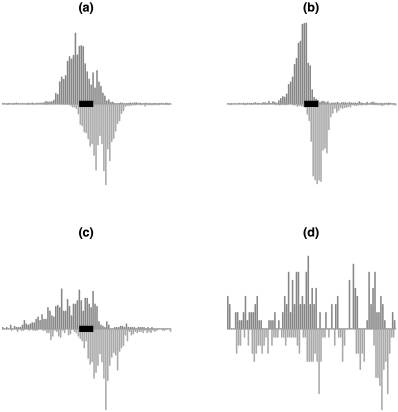
\includegraphics[width=\textwidth]{../img/peaks.jpg}
    \captionsource{Illustration of individual reads mapping to the forward (up) and reverse (down) strand, building the good bimodal binding site prfile (a, b, c) and false positive (d). }{doi: 10.1371/journal.pone.0089694}
    \label{fig:graph_classes}
\end{figure}

The computational method of the protein-chromatin binding event identification plays a central role in ChIP-seq analysis. 
After read mapping to the reference, the next step is to identify loci with high read density comparatively to the background, referred to ChIP-seq signals, or simply peaks.
More than 30 algorithms and tools have been implemented to solve that computational problem~\cite{chen2012systematic}.
The choice of the right peak caller is crucial and depends on the type of experiment~\cite{nakato2017recent}, e.g. TF binding event identification vs. long-range histone marks interactions.



Suitable software builds a peak profile along each chromosome. 
All the peak profiles can be divided into three categories~\cite{park2009chip}. 
Sharp peaks are typical for TF due to dependency on motif sequence~\cite{landt2012chip}. 
Histones have non-specific positioning on the DNA~\cite{krig2007identification}. 
Thus the peak profile is broad and can reach several kilobases. 
The third peak type is a mix of sharp and broad signals, a typical pattern for RNA polymerase II and transcription elongation factor~\cite{squazzo2006suz12, lin2011dynamic}.
% \todo{to je zavádějící. Nukleosomy sice nevážou konkrétní motiv DNA, ale vykazují jistou míru sekvenčních preferencí, která se liší v závislosti na organismu.}



The very first extended set methodology to calculate peak profile density was presented in 2007~\cite{robertson2007genome}. 
Fragments are sequenced from 5' to 3' end, and the minimal enough length of a sequenced read is 36 bp long. 
But the real fragment of DNA is longer, and thus the interaction of the protein of interest is somewhere on that size selected long DNA fragment. 
Each read is computationally extended in the 3' direction. 
Regions are scored by the number of overlap reads and assessed as a candidate peak.



Sequence directionality sets the stage for a smoothed profile. 
The strand-specific read distribution form bimodal pattern combined by shifting or extending tags toward the center~\cite{valouev2008genome}.
%% \todo{obrázek by možná čtenářům pomohl snáze pochopit popisované kroky}

%%%%%%%%%%%%%%%%%%%%%%%%%%%%%%%%%%%%%%%%%%%%%%%%%%%
\section{Statistical model utilization for the assesment of the significance of estimated signals.}


Standard biological research has some rate of false positives. 
Due to there is no absolute proof or absolute rejection of the results in ChIP-seq studies, the analysis works with probabilities.
The end goal of the ChIP-seq experiment is the genomic loci of possible protein binding events. 
The end goal of the ChIP-seq experiment is to define the genomic loci of possible protein binding events. 
The candidate signal of a binding event is represented as a hypothesis $H_{1}$, and the null hypothesis $H_{0}$ is that there is no actual binding. To describe the statistical significance of the individual hypothesis, a P-value is calculated. 

The early approach was that the background noise is uniform; 
however, the usage of the control dataset shows that the different biases make uniform model is too ideal to be true~\cite{robertson2007genome}. 
That is why all peak calling algorithms make all the output signals associated with P-value~\cite{chitpin2019recap} to determine statistical significance in a hypothesis test. 
The null hypothesis's incorrect rejection produces the Type I error known as a "false positive". 
In the contest of ChIP-seq analysis, this type of error occurs when there is no actual binding event, but the peak caller shows that there is. 
The inversion of Type I error is Type II error, which is referred to as a "false negative". 
Considering the ChIP-seq experiment, the "false negative" error type is seen less serious than "false positives". 
\todo{proč to tak je? a můžeš své tvrzení podpořit nějakou citací?}

To test peaks for significance, different peak calling algorithms adopt different statistical techniques. 
In a MUSIC's approach~\cite{harmanci2014music}, a window of fixed size for TF or varying width for histone marks while scanning a genome ranks the candidate peaks using a Binomial test, where the distribution of the total number of mapped tags in the respective regions across IP and control is assumed to be equal:

\begin{align*}
    p_{k,n} = \binom{n}{k}p^k(1-p)^{n-k}
\end{align*}

The widely used Poisson model was utilized in early software tools such as SICER~\cite{zang2009clustering}. 
The Poisson is directly connected to Binomial distribution,
where probability \textit{p} of succes in each trail and p$_{k,n}$  for \textit{k} succes in \textit{n} trails; but assosiated with rare events:

\begin{align*}
    p_{0,n} = (1 - p)^{n} = \left(1-{\frac{\lambda}{n}}\right)^{n} \to e^{-\lambda}
\end{align*}

\begin{align*}
    p_{1,n} = np(1 - p)^{n-1} = \frac{\lambda}{1-p}\left(1-{\frac{\lambda}{n}}\right)^{n} \to \lambda e^{-\lambda}
\end{align*}

\begin{align*}
    p_{2,n} = \frac{1}{2} n(n - 1) p^{2} (1-p)^{n-2} = \frac{1}{2} \frac{\lambda^{2} - \lambda p}{ (1-p)^{2}} \left(1-{\frac{\lambda}{n}}\right)^{n} \to \frac{1}{2} \lambda^{2} e^{-\lambda}
\end{align*}

For \textit{k} succes in \textit{n} trails with probability p=${\lambda / n}$ , the binomial probability p$_{n,k}$ approaches the Poisson probability:

\begin{align*}
    P_k = \frac{\lambda _i ^{k}}{k!} e^{- \lambda _i}
\end{align*}

The Poisson parameter $\lambda_i$ is supposed to be constant across the genome and provided to be inadequate for ChIP-seq peak calling to identify TFs binding sites. 
The negative binomial model was suggested by CisGenome~\cite{ji2008inte}, which is, in fact, a generalization of the Poisson distribution, also known as the gamma-Poisson mixture distribution. 

\begin{align*}
    NB_{y_i; \mu _i, \alpha} = \frac{\Gamma (y_i + \alpha ^{-1})}{\Gamma(\alpha ^{-1})\Gamma(y_i + 1)} \left(\frac{\alpha ^{-1}}{\alpha ^{-1} + \mu_i}\right) ^{\alpha ^{-1}} \left(\frac{ \mu _i}{ \alpha ^{-1} + \mu _i}\right) ^{y _i}
\end{align*}

The derevation from two-parameter gamma distribution is done in on page 118 in~\cite[Cameron and Trivedi (2013)]{cameron2013regression}.

Another suggestion was to estimate $\lambda$ for each genomic position by the local Poisson test. 
Such an approach was introduced by the most popular peak caller called MACS~\cite{zhang2008model}.
The tool slides with a constant size window centered on each nucleotide across the genome, merge overlapping peaks by extending the read.
If the number of reads in the IP sample is higher than expected, given a background rate estimated from the control dataset, then using the Poison test, the enriched regions are ranked~\cite{thomas2017features}. 
The highest tag pileup is defined as a summit of a signal.  

Comparing the statistical models implemented by different peak calling algorithms shows that the Poisson test is a better approach to score the candidate signals than the Binomial test~\cite{thomas2017features}.

%%%%%%%%%%%%%%%%%%%%%%%%%%%%%%%%%%%%%%%%%%%%%%%%%%
\section{Multiple hypothesis testing and reliability of the result.}

After scanning through the genome and find a large number of candidate regions estimating null distribution, the quality of the detected peaks should be identified. 
From generated data, the candidate signal may be either a false or true binding event. 
And the probabilistic statement cannot be made by using a well known Bayes' Theorem. 
In the genomic studies, especially in ChIP-seq, individual hypothesis testing is not useful, and a global hypothesis test is required~\cite{futschik2019omnibus}. 

Suppose we have \textit{n} genomic loci obtained.
The $i^{th}$ null hypothesis $H_{0,i}$ with corresponding P-values $p_i$.
The global null hypothesis of simultenious test of all null hypitheses  is defined:

\begin{align*}
    H_0 = \displaystyle\bigcap_{i=1}^{n} H_{0, i}
\end{align*}

Fisher's combined probability test~\cite{fisher1992statistical} combines known P-values:

\begin{align*}
    T = - \displaystyle \sum_{i=1}^{n} 2 \log p_i \sim  \chi_{2n}^{2}
\end{align*}

Bonferroni's test~\cite{hommel1988stagewise} looks at the smallest P-value and at given desired level $\alpha$ tests the global null hypothesis by testing each $H_{0,i}$ at level $\alpha /n$. 
And whenever $p_i \leq \alpha / n$ rejects the global null hypothesis.
Assuming the global hypothesis is true, the overal level control is: 

\begin{align*}
    P_{H_0}[Error Type I] = P_{H_0} \left[\bigcup_{i=1}^{n} \left\{ p_i \leq \alpha / n\right\}\right] \leq \sum_{i=1}^{n} P_{H_0}(p_i \le \alpha / n)  = n \frac{\alpha}{n} = \alpha
\end{align*}

\todo{pro Fishera a FWER chybí citace}
Even though both tests are easy and straightforward, non of them is effective. 
Fisher's test will be eliminated in a large number of the true null hypothesis. 
In the case of  Bonferroni's test, the only one P-value is used. 
Hence it can be applied only if very few binding events are expected to be significant. 
The rejection of extreme value of binding event at the $\alpha$ significance level leads to increase number of false positives. 
The idea of the global null hypothesis rejection is not suitable for genomic analysis. 
Another approach is the familywise error (FWER) rate method:

\begin{align*}
    FWER \leq 1 - (1 - \alpha)^c, 
\end{align*}

where $\alpha$ is a level for an individual test, $c$ is a number of comparisons.
The test controls the probability of performing one or more Type I errors. 
However, the method is very conservative and does only a few rejections. 

The application of the False Discovery Rate (FDR) approach in the genomic field is associated with microarray technology~\cite{lai2017statistical}.
The method allows a few small rejections if the majority of the rejections are correct. 
\todo{nerozumím, co znamená "SMALL rejection"}
Such testing adjusts the statistical confidence based on the number of tests. 

Let $R$ be the total number of rejections and $V$ be the number of trully null hypotheses.
The the proportion $Q$ of false positive rejection among all rejection is 

\begin{align*}
    Q = \frac{V}{R} .
\end{align*}

The Benjamini-Hochberg procedure~\cite{benjamini2000adaptive} ensures the expectetion and define False Dicovery Rate as follow: 

\begin{align*}
    FDR = E(Q) = E \left(\frac{V}{R}\right) .
\end{align*}

If all null hypotheses are true, then FDR and FWER are indeed the same.
The most common significance level accepted is 95, which means that 95\% of the obtained result has a chance to be true. 
The p = 0,05 cutoff means that the chance of making a wrong decision is equal to 5\%. 
It is too strict and leads to the loss of a real finding. 
That is why the q-value was introduced to calibrate the false discovery rate measurements~\cite{storey2003statistical}. 
P-value test the significance of the false-positive rates and the q-value test the significance in term of false discovery rate. 
In other words, the threshold choice either by P- or q-value should be based on how many false positives are expected in the experiment.



%%%%%%%%%%%%%%%%%%%%%%%%%%%%%%%%%%%%%%%%%%%%%
\section{Statistical sin}

Most programs for identification of the enriched regions (peaks) work as follow: candidate signal are identified by analyzing along the genome, and then by comparing with the input or mock dataset(or with another IP data in case of the differential analysis) regions are evaluated. 
However, most of the software tools use data twice to identify and assess the enrichment, which leads to a statistical sin~\cite{lun2014novo}. 
Moreover, the estimated P-values depend on the same data and result in statistical bias.
A similar problem can influence the result during ChIP-seq analysis and in areas such as DNA variant calling~\cite{chitpin2019recap}.

Without a correctly calculated P-value, it is difficult to choose the right cutoff threshold, which influences the final results. 
Improper P-values lead to difficulties in evaluating of reliability of a given set of peaks.
It may also lead to loss of the true binding event due to the biased statistical significance of such a peak, and further downstream analysis will exhibit the error-prone result~\cite{chitpin2019recap}. 

A possible solution to that problem is to develop a new peak identification approach to avoid double usage of the same data. 
However, many software tools are good enough to be used, and recalibration of the obtained P-values is the possible alternative resolve~\cite{chitpin2019recap}.

%%%%%%%%%%%%%%%%%%%%%%%%%%%%%%%%%%%%%%%%%%%%
\section{Reliability of the obtained list of ChIP-seq signals after peak calling procedure.}

Peak identification process outputs typically tens of thousands of possible binding loci, which are needed to be assessed. 
An obtained list of peak coordinates may be annotated with the nearest gene. 
However, the lack of annotated actual binding sites may limit the process of the validation of the experiment result~\cite{nakato2017recent}.

The motif-discover of a peak collection is another available approach. 
Typically the top-ranked by P-value identified peaks are undergoing the motif finding procedure~\cite{bailey2011dreme}.
Motifs are represented as a position weight matrix and sequence logo and suitable for the TF experiment due to the specificity of the binding protein.
However, for the proteins which bind without a preferable sequence such as histones, the motif-based evaluation of the peak reliability is not suitable~\cite{nakato2017recent}. 

If more than one biological replicates are available, then another way to validate signals is to assess the global similarity between replicates with a calculation of the cross-correlation coefficient. 
IDR, which validates the rank consistency of common peaks in replicates, is another way for the peak validation, which may help to filter out false-positive peaks. 

As  was mentioned, the bimodal peak pattern is utilized in peak calling design. 
Many false positives may be filtered out by analyzing the size and appearance of the signal~\cite{rye2011manually}. 
However, only a few methods utilize the analysis of the peak shapes~\cite{hower2011shape, wu2014polyapeak}.



 %The directionality of the sequencing reads produces bimodal enrichment on both strands centered around the binding site of the protein of interest. The cross-correlation metric can evaluate each obtained peak. The calculation is based on Pearson's linear correlation between forward and reverse strand for each complementarity base by shifting minus strand. The procedure generates two peaks, a bigger on corresponding to the fragment length, and a smaller one is associated with a read length. 
\chapter{bias, artefacts}

% To ensure reliability of the data, at least duplicate biological replicate experiments should be done.
% Sonication of crosslinked chromatin may be preffered method.
% Mocrococcal nuclease degrade linker DNA where TF tend to bind.
% The conditions of sonication should be optimized for each cell type.
% Because they depend on cell type, type of sonicator and  sonicator settings.

\section{assay artefacts}
Strong enrichment signals suggestive of proteins binding to genomic loci where genes were higly transcribed were found.
Moreover, the enrichment for proteins binding to higly-transcribed genes was was observed even in controls like moch ChIP-seq data.
Which poins to an overall bias that could contaminate any ChIP-seq data with false positives~\cite{park2013widespread}
A secondary bias of nucleosomal periodicity was also commonly observed across ChIP-seq dataset.
And contributed additional false positives in which proteins falsly appeared to interact with nucleosomes.

Two features among strong false positive signals.
First, the signals were present within gene bodies.
Second, Stronges signal derived from genes thet are known to be higly expressed.

% It is possible that certain TF trully bind to ORFas a means of regulating gene expression.
A common use of ChIP-seq is to examine binding of a given factor under different growth conditions or backgrounds.
Since only a single variable is changed (growth condition), it might be assumed that comparing binding under different conditions offers a reliable means of identifying biologically relevant targets, with most background artefacts being ormalized out.

One bias arised during genome sonication.
Open chromatin regions are easely shared than other regions.
Thus these open regions yield more protein-DNA complexes.
IP step immunoprecepitate more complexes from the open chromatin regions.
And as a result gives more sequenced reads.

To correct this bias, the fragmented genome are divided into two portions.
One portion goes through the IP step.
And then sequenced.
Other portion is sequenced directly.
This portion serve the input control.

This input control can be used to normalize the shearing bias of sonication~\cite{kharchenko2008design}.
% Type of normalization controls might be appropriate for normalizing false positives?

In the analysis of ChIP-seq data two types of normalization or correction controls are commonly used.

The input sample has the advanage that all the regions of the genome are well represented.
The sample concentration is ample and stable for constructing sequencing libraries.
The same sample can potentially serve as the control for several related experiments.

The input a baseline signal for reads across the genome, factoring in sequence mappability and copy number differences relative to the reference genome.
For these reasons, input has been suggested as a more effective control.

However, genes transcribed at high rates is not adequately represented in the input.

A mock ChIP is designed to correct data with large quantity of spurious sites in ChIP-seq, which are coused by uneven genomic sonication and nonspecific interactions between chromatin and antibody.
\todo{nezapomeň na nespecifické interakce mezi chromatinem a magnetickými/polysacharidovými kuličkami, které se používají pro purifikaci komplexů chromatin-protilátka}
Whereas DNA input controls corrects only for uneven sonication.
\todo{řekl bych, že input dokáže korigovat i PCR amplification bias (GC bias?)}

Mock better reflects the background enrichment from highly transcribed genes.
Mock ChIP-seq data exhibit a stronger expression bias than the corresponding input sample.
Therefore correction by mock ChIP (normalization) would be more effectively reduce the false-positives than normalization by input~\cite{park2013widespread}.
Mock ia s better control for minimizing the appearence of occupancy signal over transcribed regions.
\todo{mock IP má ale tendenci precipitovat jen velmi malé množství chromatinu (DNA), které je do určité míry náhodné a tedy nereproducibilní. Při PCR pak dochází k overamplifikaci.}

Measuring the binding of a TF under two different conditions and identifying the differentially bound target offers the most reliable way to identify targets of biological significence.
\todo{s tímhle nesouhlasím, je to příliš obecně definované. Pokud například opůsobím buňky nějakým inhibitorem, který do 10 min způsobí disociaci TF z chromatinu, tak se to na transkripci moc neprojeví a artefakty mi zůstanou prakticky stejné.}
The assumption that most sources of background signal are canseled out between two samples is risky.
Expression biase derives directly from actively transcribed genes.
Transcription will differ between two conditions.
\todo{není jisté, zda se bude transkripce mezi podmínkami lišit. Záleží, jaké to jsou podmínky. A určitě bude existovat nějaká skupina vysoce exprimovaných housekeeping genů, které budou silně transkribované za obou podmínek: např. proteiny translačního aparátu, cytoskelet atd.}
Even in these cases ChIP data from each condition has to be properly corrected by the corresponding mock ChIP data to minimize false positives.

% CROSSLINK
% ===========
\section{Non-specific TF interactions, crosslinking time}

ChIP-seq technology has been used to identify the localization of post-translationally modified histones, histone variants, TF, and other chromatin-associated proteins.
Native ChIP is commonly used for the analysis of stable chromatin complexes~\cite{kasinathan2014high} and histones.
Transcription factor interactions that would not withstand the isolation procedure due to weak affinity to the DNA require a crosslinking step.
% \todo{"native" bych zde nepoužíval, spíš specific nebo genuine. Nativní se používá jako protiklad k fixovaný (např. native vs formaldehyde-fixed ChIP)}


Typical ChIP assay involves crosslinking using formaldehyde reactivity. 
This smallest aldehyde has been applied for decades in numerous fields~\cite{eckels2003formalin,werner2000effect,gavrilov2015vivo}.
In the chromatin immunoprecipitation, the ability of formaldehyde to crosslink with proteins and DNA to form protein-DNA or protein-protein complexes provides identification of the location of transcription factor binding along the DNA strand.
Cell permeability, short spacer length, rapid reactivity, and reversibility are key properties that define formaldehyde as a crosslinking fixative of choice for ChIP~\cite{hoffman2015formaldehyde}.

Unlike other essential regulatory proteins, transcription factors contain at least one DNA-binding domain that contains at least one structural motif that specifically recognizes dsDNA or ssDNA~\cite{mitchell1989transcriptional}.
Some transcription factors bind non-specifically~\cite{struhl2007interpreting};
and it is also known, that site-specific TFs can bind non-specifically~\cite{hammar2012lac,mirny2009protein} but with weaker affinity.

Several studies show that different DNA-binding proteins spend some time non-specifically bound and sliding along DNA~\cite{slutsky2004kinetics,mirny2010nucleosome,cherstvy2008protein,hu2006proteins,sheinman2009effects}.
And the approach is that the search process is a combination of three-dimensional and one-dimensional diffusion and also can be statistically predicted~\cite{sela2011dna}.
Such non-specific accessibility of the genome in different regions leads to the non-specific cross-linking events, which can increase the rate of false-positive signals in further analysis.

The formaldehyde concentration, incubation time, and other conditions can vary from experiment to experiment. 
Even though the effective crosslinking time is of the 5-second threshold~\cite{schmiedeberg2009temporal}, many laboratories use rather prolonged formaldehyde incubation time.
Soluble proteins not expected to associate with DNA would be non-specifically captures at the open chromatin loci.

Soluble proteins not expected to associate with DNA would be non-specifically captures at the open chromatin loci. Shortening the incubation time traps preferentially genuine DNA-protein binding events~\cite{baranello2016chip}.



% GC bias
% ============
\section{GC content bias in ChIP-seq is challenging}
Effective analysis requires sufficient coverage by sequence reads. 
The sequenced reads must overlap to achieve the required level of resolution for a ChIP experiment.
Whereby the experiment requires many copies of a whole genome.
Nowadays ChIP purified DNA is obtained from many cells.
Multiple genome copies provide a sufficient number of overlapping reads after cleavage and sequencing.
In addition, sigle-cell sequencing requires PCR-amplification before the fragmentation step~\cite{clark2016single}.

% \todo{důležitá poznámka k celému odstavci: DNA/chromatin se u ChIPu fragmentuje pouze před imunoprecipitací. Poté, co vyizoluješ čistou DNA, se už žádná další fragmentace neprovádí. Rovnou se připraví knihovna a sekvenuje se!}

The coverage for ChIP-seq varies across experiments due to GC-content bias, and that variability may introduce false-positive signals during downstream analysis.
Loci with high GC base composition are often under-represented, and such bias has been observed in several NGS experiments~\cite{benjamini2012summarizing,dohm2008substantial,teng2017accounting}.
This bias tends to have appeared during the PCR amplification~\cite{ross2013characterizing}.
It is known that GC-rich DNA targets are less amenable to amplification due to base base-stacking interations~\cite{yakovchuk2006base}.
% \todo{GC bias vzniká také v průběhu PCR, kdy se GC-rich fragmeny amplifikují hůře než GC-poor. Je to dáno jejich méně efektivní denaturací - mají vyšší vazebnou energii}

Both PCR amplification during library construction and PCR for cluster amplification on the Illumina platform play role. 
The first case has many potential solutions to avoid the bias during library construction step.
It requires preparing a larger amount of the input DNA to avoid PCR itself, or PCR step with extensive optimization such as annealing time and temperatures and primer specifity~\cite{aird2011analyzing}.
The possible problem of Illumina cell flow bridge amplification may occur due to secondary structures.
GC-rich sequences form hairpins, which are stable and stack unmelted at usual PCR denaturation temperatures~\cite{stein2010nucleosome}.

Fragmentation is the first step in DNA sequencing process.
This step ensures the solubility of the crosslinked DNA-protein complexes are soluble and accessible to antibody.
Using enzymatic digestion, chemical shearing, or different mechanical method, DNA with crosslinked proteins is broken up into short fragments.
After immunoprecipitation one or both ends of the fragment sequenced.


The early assumption was that genomic DNA break randomly.
However, the experiment~\cite{poptsova2014non} with different methods of DNA fragmentation showed that the rates of double-stranded breaks are sequence-dependent.
This dependency may also cause the GC-bias. 

However, true binding sites of the protein of interest may be expected to occur in high GC regions.
% \todo{"are expected" -> spíš "may be expected"}\todo{. Oblasti vazby vůbec nemusí být GC-bohaté, záleží na cílovém proteinu}
Those regions have biological relevance such as promotor regions.
Modeling of the GC-content at the fragment level~\cite{benjamini2012summarizing} is the optimal approach, but is not directly applicable to ChIP-seq analysis.
The method for correction of this kind of bias was presented~\cite{teng2017accounting}.
Incorporation of the approach into current peak callers shows substantial improvements in signal finding.
However, the method is not suitable for broad peak identification as histone modifications.






% Blacklist
% ============
\section{Blacklist region/Difficulties in the ussambly/overrepresented regions}

Signals based on high-throughout sequencing output rely on an accurate genomic annotation and mapping.
In some regions, such as regions with a large number of structural variants and repetitive regions, the assembly of the genome can be difficult and may may be collapsed or under-represented relative to the actual underlying genomic sequence.
Problems with the assembly have effects on the mapping and calling and lead to inaccurate interpretation of the downstream analysis.
Duplication rate for single-end ChIP-seq data is overestimated and leads to ChIP-seq signal being lost within those regions~\cite{chen2012systematic}.


\chapter*{Conclusion}
\addcontentsline{toc}{chapter}{Conclusion}


%%% Bibliography
%%% Bibliography (literature used as a source)
%%%
%%% We employ bibTeX to construct the bibliography. It processes
%%% citations in the text (e.g., the \cite{...} macro) and looks up
%%% relevant entries in the bibliography.bib file.
%%%
%%% The \bibliographystyle command selects, which style will be used
%%% for references from the text. The argument in curly brackets is
%%% the name of the corresponding style file (*.bst). Both styles
%%% mentioned in this template are included in LaTeX distributions.

% \bibliographystyle{plainnat}    %% Author (year)
 \bibliographystyle{unsrt}     %% [number]

\renewcommand{\bibname}{Bibliography}

%%% Generate the bibliography. Beware that if you cited no works,
%%% the empty list will be omitted completely.

\bibliography{bibliography}

%%% If case you prefer to write the bibliography manually (without bibTeX),
%%% you can use the following. Please follow the ISO 690 standard and
%%% citation conventions of your field of research.

% \begin{thebibliography}{99}
%
% \bibitem{lamport94}
%   {\sc Lamport,} Leslie.
%   \emph{\LaTeX: A Document Preparation System}.
%   2nd edition.
%   Massachusetts: Addison Wesley, 1994.
%   ISBN 0-201-52983-1.
%
% \end{thebibliography}


%%% Figures used in the thesis (consider if this is needed)
\listoffigures

%%% Tables used in the thesis (consider if this is needed)
%%% In mathematical theses, it could be better to move the list of tables to the beginning of the thesis.
\listoftables

%%% Abbreviations used in the thesis, if any, including their explanation
%%% In mathematical theses, it could be better to move the list of abbreviations to the beginning of the thesis.
\chapwithtoc{List of Abbreviations}

%%% Attachments to the bachelor thesis, if any. Each attachment must be
%%% referred to at least once from the text of the thesis. Attachments
%%% are numbered.
%%%
%%% The printed version should preferably contain attachments, which can be
%%% read (additional tables and charts, supplementary text, examples of
%%% program output, etc.). The electronic version is more suited for attachments
%%% which will likely be used in an electronic form rather than read (program
%%% source code, data files, interactive charts, etc.). Electronic attachments
%%% should be uploaded to SIS and optionally also included in the thesis on a~CD/DVD.
%%% Allowed file formats are specified in a provision of the rector no. 72/2017.
\appendix
\chapter{Attachments}

\section{First Attachment}
s
\openright
\end{document}
